\documentclass[autodetect-engine,dvipdfmx-if-dvi,ja=standard]{bxjsarticle}

% 二段組にするとき
% \documentclass[twocolumn,autodetect-engine,dvipdfmx-if-dvi,ja=standard]{bxjsarticle}

\usepackage{graphicx}        %図を表示するのに必要
\usepackage{color}           %jpgなどを表示するのに必要
\usepackage{amsmath,amssymb} %数学記号を出すのに必要
\usepackage{setspace}
\usepackage{eclclass}
\usepackage{cases}
\usepackage{here}
\usepackage{fancyhdr}
\usepackage{ascmac}

% 文書全体のスタイルを設定(主に余白)
\setlength{\topmargin}{-0.3in}
\setlength{\oddsidemargin}{0pt}
\setlength{\evensidemargin}{0pt}
\setlength{\textheight}{44\baselineskip}

% 行頭の字下げをしない
\parindent = 0pt

% ヘッダとフッタの設定
\lhead{電気情報工学応用実験II}
\chead{}
\rhead{5E 20番 佐藤凌雅}
\lfoot{}
\cfoot{-\thepage-} % ページ数
\rfoot{}

% 式の番号を(senction_num.num)のようにする
\makeatletter
\@addtoreset{equation}{section}
\def\theequation{\thesection.\arabic{equation}}
\makeatother

% 画像の貼り付けを簡単にする
\newcommand{\pic}[2]
{
  \begin{figure}[H]
    \begin{center}
      \includegraphics[scale=#2]{#1}
    \end{center}
  \end{figure}
}

% 単位の記述を簡単にする
\newcommand{\unit}[1]
{
  \, [\mathrm{#1}]
}
\begin{document}
% \maketitle
\pagestyle{fancy}
\section{目的}
太陽電池の各試験を行い,太陽電池の特性を知り,取り扱い上の要点を習得する.\\

\section{理論}
\subsection{再生可能エネルギー}
 太陽光,風力,その他非化石エネルギー源のうち,エネルギー源として永続的に利用することができると認められるもののこと.\\
 再生可能エネルギーとして,太陽光,風力,水力,地熱,太陽熱,大気中の熱その他の自然界に存する熱,バイオマスが挙げられる.
\footnote{環境省 平成26年度2050年再生可能エネルギー等分散型エネルギー普及可能性検証検討委託業務報告書 第1章再生可能エネルギー導入加速化の必要性,https://www.env.go.jp/earth/report/h27-01/,2019-7-1閲覧}


\subsection{太陽光発電の原理}
 現在最も多く使われている太陽電池は,シリコン系太陽電池である.この太陽電池では,電気的な性質の異なる2種類(p型,n型)の半導体を重ね合わせた構造をしている.\\
 太陽電池に太陽の光が当たると,電子と正孔が発生し,正孔はp型半導体へ,電子はn型半導体側へ引き寄せられる.このため、表面と裏面につけた電極に導線をつなげば,電子がn型からp型に,正孔はp型からn型に流れ,電流を取り出すことができる.
\footnote{太陽電池とは - 太陽光発電協会,http://www.jpea.gr.jp/knowledge/solarbattery/index.html,2019-7-1閲覧}
\begin{figure}[H]
  \centering
  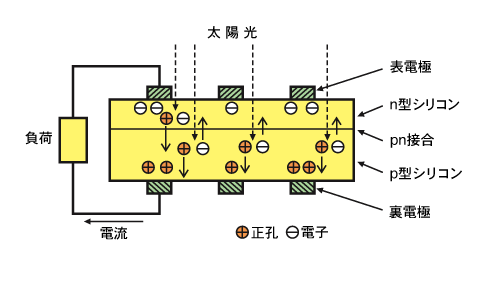
\includegraphics[width=13cm]{./fig/fig01.png}
  \caption{太陽光発電の原理}
\end{figure}

\subsection{種類}
太陽光発電の種類は,使用している材料によって細かく分けられているが,大別すると図.2のようになる.\\
\begin{figure}[H]
  \centering
  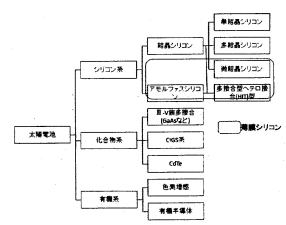
\includegraphics[height=7cm]{./fig/fig02.png}
  \caption{太陽光発電の種類}
\end{figure}

\section{実験装置回路}
\begin{figure}[H]
  \centering
  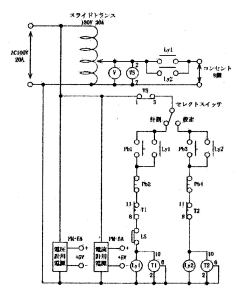
\includegraphics[height=7cm]{./fig/fig03.png}
  \caption{実験装置回路}
\end{figure}


\section{使用機器}
太陽電池実験装置\\
照度計\\

\section{実験方法}
\bf{測定上の注意}\\
 実験装置のセレクトスイッチは以下の特性を持っているので,測定の際はすばやく読み取ること.\\
 設定:太陽電池がセットされていなくても,「ON」にしたときランプが約 30 秒点灯する. \\
 測定:太陽電池がセットされている場合に限り,約5秒点灯する.\\

\subsection{開放電圧の照度依存性試験}
\begin{enumerate}
  \item 実験装置のコンセントを差し込む前に以下の設定を行う.\\
  ・負荷スイッチは「OFF」にする.\\
  ・ スライドトランスは「0」にする.
  \item 照度計を太陽電池脇のほぼ中心にセットする.以降,照度計は極力動かさないこと.
  \item セレクトスイッチを設定にセット,装置の照明を ON にすることで,照度の設定ができる.100lx が理想だが,実験室の原明を感知するときがあるので,その時は最低値に設定する.
  \item セレクトスイッチを測定にセット,装置の照明を ON にすることで,各数値を読むことができる.この項目では発生電圧を読み取る.
  \item 照度を対数的に上げていき同様の測定を行う(最高照度は 20000lx).
\end{enumerate}


\subsection{短絡電流の照度依存性試験}
\begin{enumerate}
  \item 以下の設定を行う.\\
  ・ 負荷スイッチは「ON」にする.\\
  ・負荷抵抗は「100\%」にする.\\
  ・ スライドトランスは「0」にする.
  \item 照度の設定は,5.1 と同様に行い,発電電流を読み取る.
\end{enumerate}


\subsection{電圧電流特性の照度依存性試験}
\begin{enumerate}
  \item 以下の設定を行う.\\
  ・ 負荷スイッチは「ON」にする.\\
  ・ 負荷抵抗は「0\%」にする.\\
  ・スライドトランスは「0」にする.
  \item 照度の設定は,5.1 を参照.
  \item 一定限度のもと,負荷抵抗を 0\% から 100\%まで増加し,それぞれの発電電圧および発電電流を読み取る.
\end{enumerate}



\end{document}
